$y=4x-x^2$, $y=0$, $x=1$, $x=3$

\nopagebreak
\begin{align*}
\text{La parábola } y=4x-x^2 \text{ corta al eje } x \text{ en } x=0, x=4. \\
\text{En } [1,3], y \ge 0. \\
A &= \int_{1}^{3} (4x-x^2) \, dx = \left[ 2x^2 - \frac{x^3}{3} \right]_{1}^{3} \\
&= (18 - 9) - (2 - 1/3) \\
&= 9 - 5/3 = 22/3
\end{align*}

\[
\boxed{\displaystyle \frac{22}{3}}
\]

\begin{center}
    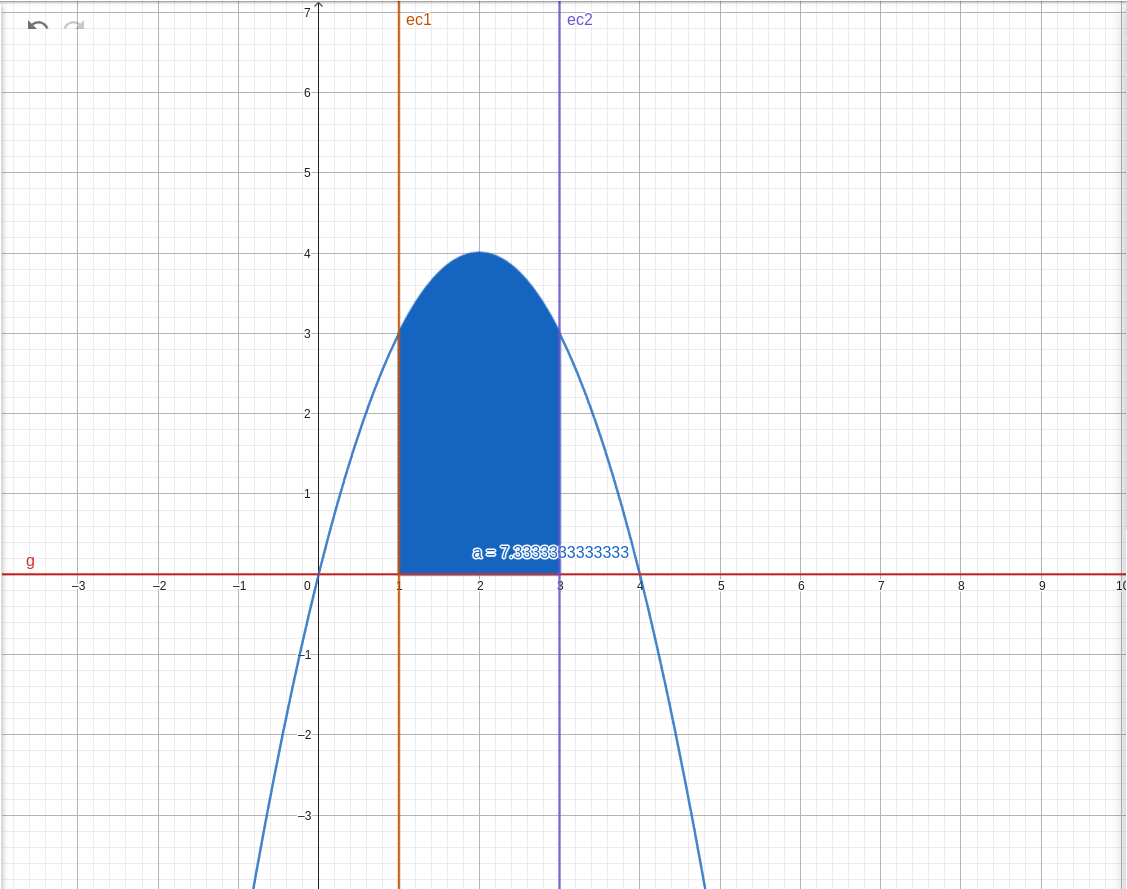
\includegraphics[width=0.5\textwidth]{Graficas/ejer17.png}
\end{center}
